\chapter{Proposed System}
\label{chapter:proposed system}
\quad The aim of this projecct is to build a Linux capable RISC-V-based SoC using IOb-SoC. IOb-SoC already has a RISC-V CPU, picorv32, but this processor isn't capable of running Linux.
\begin{figure}
  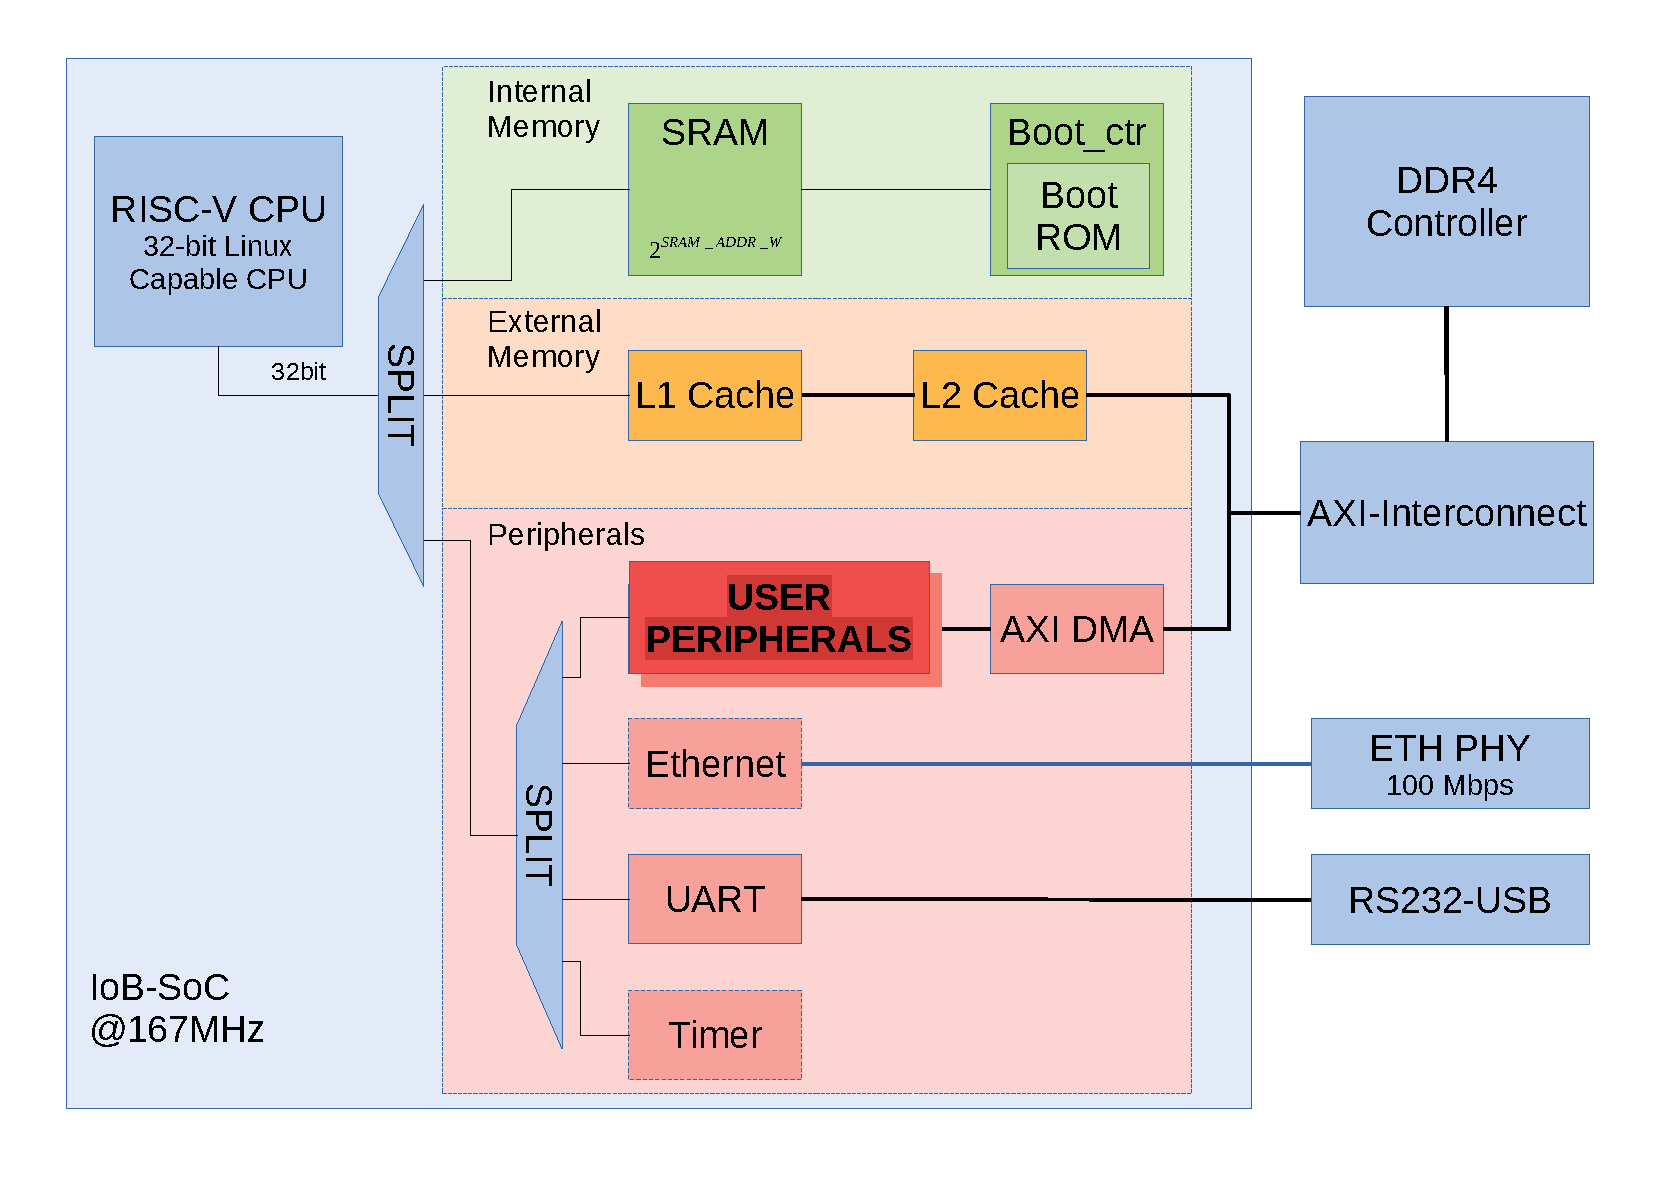
\includegraphics{Figures/bd.pdf}
  \caption{Modular hardware arquitecture of the proposed system}
  \label{fig: IOb-SoC modules}
\end{figure}

\section{CPU selection}
\quad When chosing which CPU should be implemented on the IOb-SoC in order to be able to run Linux on it some specification need to be taken into consideration.
Supported architectures are rv32i or rv64i plus standard extensions (a)tomics, (m)ultiplication and division, (f)loat, (d)ouble, or (g)eneral for MAFD. And C stands for compact.

\subsection{BOOM}
\quad The Berkeley Out-of-Order Machine (BOOM) is a synthesizable and parameterizable open source RV64GC RISC-V core written in the Chisel hardware construction language. While BOOM is primarily ASIC optimized, it is also usable on FPGAs. It was created at the University of California, Berkeley in the Berkeley Architecture Research group, its focus is to create a high performance, synthesizable, and parameterizable core for architecture research.

\quad Pros:
\begin{itemize}
  \item Extensive Instrution Set arquitecture s
\end{itemize}
\quad Cons:
\begin{itemize}
  \item 64-bit arquitecture
  \item writen in Chisel
  \item ASIC optimized
\end{itemize}

\subsection{CVA6/Arianne}
\quad CVA6 is a 6-stage, single issue, in-order CPU which implements the 64-bit RISC-V instruction set. It fully implements I, M, A and C extensions as specified in Volume I: User-Level ISA V 2.3 as well as the draft privilege extension 1.10. It implements three privilege levels M, S, U to fully support a Unix-like operating system.

\quad Pros:
\begin{itemize}
  \item
\end{itemize}
\quad Cons:
\begin{itemize}
  \item 64-bit arquitecture
  \item not modular
\end{itemize}

\subsection{VexRiscv}
\quad VexRiscv CPU, a 32-bits Linux Capable RISC-V CPU written in Spinal HDL

\quad Pros:
\begin{itemize}
  \item 32-bit arquitecture
\end{itemize}
\quad Cons:
\begin{itemize}
  \item
\end{itemize}


\section{Creation of an embedded Linux image}
\quad Linux repository to create kernel, Busybox to create basic application layer, emulating using Qemu

\section{Expected system requirements}
\quad Silicon Area (ASIC mm2; FPGA #LUTs, #BRAM, #DSPs), Max Freq (ASIC/FPGA)
\subsection{LitexSoC}
